\documentclass[12pt]{article}
\usepackage{preamble}

\pagestyle{fancy}
\fancyhead[LO,LE]{Математическая статистика}
\fancyhead[RO,RE]{Лекции Блаженова А. В.}

\fancyfoot[L]{\scriptsize исходники найдутся тут: \\ \url{https://github.com/pelmesh619/itmo_conspects} \Cat}

\renewcommand{\thesection}{}

\begin{document}

    \tableofcontents
    \clearpage

    % begin mathstat_2025_02_11.tex





\section{Лекция 1.}

Теория вероятности изучает характеристику случайных величин, тогда как математическая статистика решает обратную задачу

Допустим, что у нас есть случайная величина, по ней мы можем найти матожидание, моменты и оценить,
какое распределение имеет случайная величина. 

\subsection{Выборки}

\Def \textbf{Выборка} - набор данных, полученных в ходе экспериментов. Тогда количество экспериментов $n$ - объем Выборки

\Defs \textbf{Генеральной совокупностью} называются все результаты проведенных экспериментов

\Defs \textbf{Выборочной совокупностью} называются наблюдаемые данные экспериментов

Не все данные экспериментов мы можем наблюдать, например, выборы, тогда опросы голосовавших - выборочная совокупность, а
результаты выборов - генеральная. Очевидно, что выборочная и генеральная совокупности могут иметь различные распределения.

\Defs Выборка называется \textbf{репрезентативной}, если ее распределение близко к распределению генеральной совокупностью

Пример - \href{https://ru.wikipedia.org/wiki/%D0%A1%D0%B8%D1%81%D1%82%D0%B5%D0%BC%D0%B0%D1%82%D0%B8%D1%87%D0%B5%D1%81%D0%BA%D0%B0%D1%8F_%D0%BE%D1%88%D0%B8%D0%B1%D0%BA%D0%B0_%D0%B2%D1%8B%D0%B6%D0%B8%D0%B2%D1%88%D0%B5%D0%B3%D0%BE}{ошибка выжившего}. Во время Второй Мировой стал вопрос, в каких местах стоит бронировать корпус самолета. Самолеты 
возвращались с пулевыми отверстиям, и интуитивно казалось, что стоит бронировать те места, которые больше
всего пострадали. Однако не были учтены те самолеты, которые не вернулись, а те, которые выжили, выжили благодаря тому, что были 
прострелены в нелетальных местах, поэтому было принято решение бронировать фюзеляж в менее пострадавших местах

В дальнейшем считаем, что все выборки репрезентативны

\DefN{1} Выборкой объема $n$ называется набор из $n$ экспериментаных данных $\vec{X} = (x_1, x_2, \dots, x_n)$ (апостериорное определение)

\DefNs{2} Выборкой объема $n$ называется набор из $n$ независимых одинаково распределенных случайных
величин $\vec{X} = (X_1, X_2, \dots, X_n)$ (априорное определение)

\subsection{Выборочные характеристики}

Можно выборку рассматривать как дискретную случайную величину с одинаковыми вероятностями $p_i = \frac{1}{n}$
и вычислить для нее математическое ожидание, дисперсию и функцию распределения

\Def Выборочным средним $\overline{x}$ называется величина $\overline{x} = \frac{1}{n} \sum_{i = 1}^n X_i$

\Defs Выборочной дисперсией $D^*$ называется величина $D^* = \frac{1}{n} \sum_{i = 1}^n (X_i - \overline{x})^2$ (или $D^* = \frac{1}{n} \sum_{i = 1}^n X_i^2 - \overline{x}^2$)

По закону больших чисел выборочное среднее будет сходиться к матожиданию

\Defs Исправленной дисперсией называется величина $S^2 = \frac{n}{n - 1} D^* = \frac{1}{n - 1}\sum_{i = 1}^n (X_i - \overline{x})^2$

\Def Выборочной функцией распределения $F^*(x)$ называется функция $F^*(x) = \frac{\text{число данных } x_i < x}{n}$

\begin{MyTheorem}
    \Ths Выборочная функция распределения поточечно сходится к теоретической функции распределения:

    \[\forall y \in \Real F^*(y) \overset{p}{\longrightarrow} F(y)\]
\end{MyTheorem}

\begin{MyProof}
    $F(y) = P(X < y)$

    $F^*_y = \frac{1}{n} \sum_{i = 1}^n I(X_i < y) \underset{\text{по ЗБЧ}}{\overset{p}{\longrightarrow}} EI(X_i < y) = P(X_i < y) = 
    P(X_1 < y) = F_{X_1}(y)$
\end{MyProof}

Усилим теорему

\begin{MyTheorem}
    \ThNs{Гливенко-Кантелли} $\sup_{x \in \Real} |F^*(x) - F(x)| \overset{p}{\longrightarrow} 0$
\end{MyTheorem}

\begin{MyTheorem}
    \ThNs{Колмогорова} $\sqrt{n} \sup_{x \in \Real} |F^*(x) - F(x)| \rightrightarrows K$ - распределение Колмогорова с 
    функцией распределения $F_K(x) = \sum_{j = -\infty}^{\infty} (-1)^j e^{-2 j^2 x^2}, \ x \in [0;\infty)$
\end{MyTheorem}

\subsection{Начальная обработка статданных}

\begin{enumerate}
    \item Ранжирование данных - упорядочиваем выборки по возрастанию. В результате получаем вариационный ряд $\vec{X} = (X_{(1)}, X_{(2)}, \dots, X_{(n)})$

    $X_{(1)} = \min X_i; \quad X_{(n)} = \max X_i$

    $X_{(i)} = i$-ая порядковая статистика

    \item Объединим повторяющиеся данные - получаем т.н. частотный вариационный ряд

    \begin{tabular}{c|c|c|c|c}
        $X_i$ & $X_{(1)}$ & \dots & $X_{(r)}$ & $\sum$ \\ 
        \hline
        $n_i$ & $n_1$ & \dots & $n_r$ & $n$ \\ 
    \end{tabular}

    Иногда часть данных отбрасывается сверху и снизу (по 5, по 10, по 5\% и так далее), чтобы сделать выборку репрезентативной

    Тогда $\overline{x} = \frac{1}{n} \sum X_i n_i$, $D^* = \frac{1}{n} \sum (X_i - \overline{x})^2 n_i$
    
    \item Чтобы уменьшить количество вычислений или сделать гистограмму, делают интервальный вариационный ряд: 
    разбиваем данные на интервалы и считаем, сколько данных $n_i$ попало в интервал. 

    Тогда $n_i$ - частота интервала $A_i$

    Есть два основные способа разбиения на интервалы: 

    \begin{enumerate}
        \item Интервалы одинаковой длины
        \item Равнонаполненные интервалы (в каждом интервале примерно одинаковое количество данных)
    \end{enumerate}

    Число интервалов $K$ такое, что $\frac{K(n)}{n} \longrightarrow 0$ и $K(n) \underset{n \to \infty}{\longrightarrow} \infty$

    Обычно применяют формулу Стерджесса $K \approx 1 + \log_2 n$ или $K \approx \sqrt[3]{n}$

    Пусть получили интервальный вариационный ряд

    \begin{tabular}{c|c|c|c|c|c}
        интервалы & $[a_0; a_1)$ & $[a_1; a_2)$ & \dots & $[a_{K - 1}; a_K]$ & $\sum$ \\ 
        \hline
        частоты & $n_1$ & $n_2$ & \dots & $n_K$ & $n$ \\ 
    \end{tabular}

\end{enumerate}

\subsection{Геометрическая интерпретация данных}

% https://www.geogebra.org/calculator/rcgr7r9f

\begin{itemize}
    \item Гистограмма

    Строится ступенчатая фигура из прямоугольников, основание $i$-ого прямоугольника - интервал, 
    высота прямоугольника - $\frac{n_i}{n l_i}$, где $l_i$ - длина интервала

    \begin{center}
        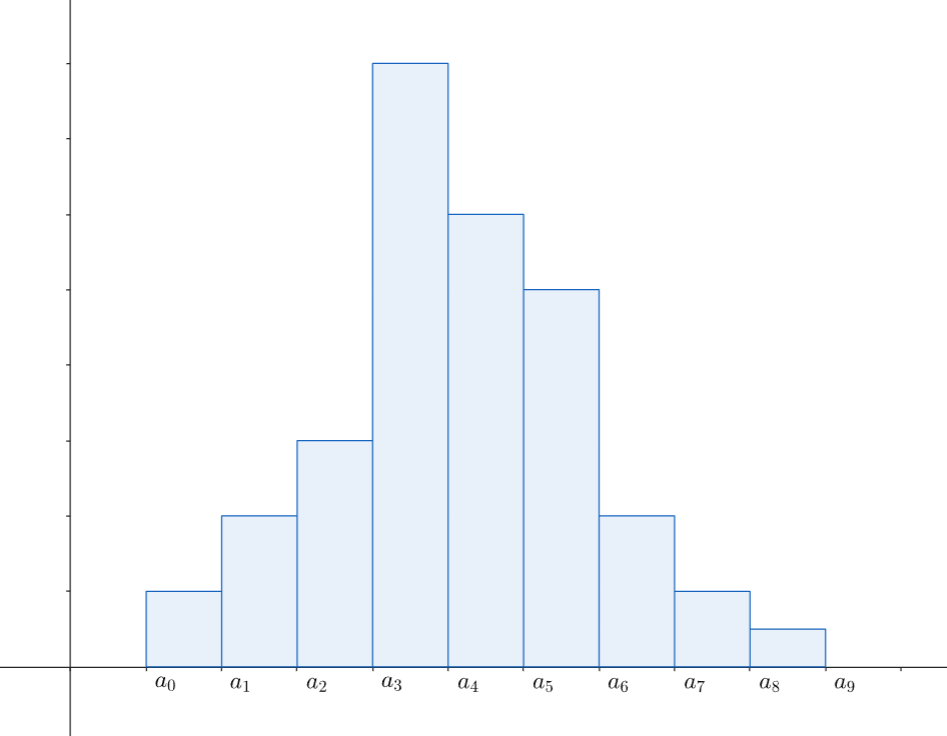
\includegraphics[width=0.7\textwidth]{mathstat/images/mathstat_2025_02_11_1}
    \end{center}

    Визуально можно сделать гипотезу, как ведет себя распределение. 

    \begin{MyTheorem}
        \Ths Гистограмма поточечно сходится к теоретической плотности
    \end{MyTheorem}

    \item Полигон

    На оси абсцисс отмечаем значения частотного вариационного ряда, по оси ординат - их частоты. 
    Получившиеся точки соединяем отрезками

    \begin{center}
        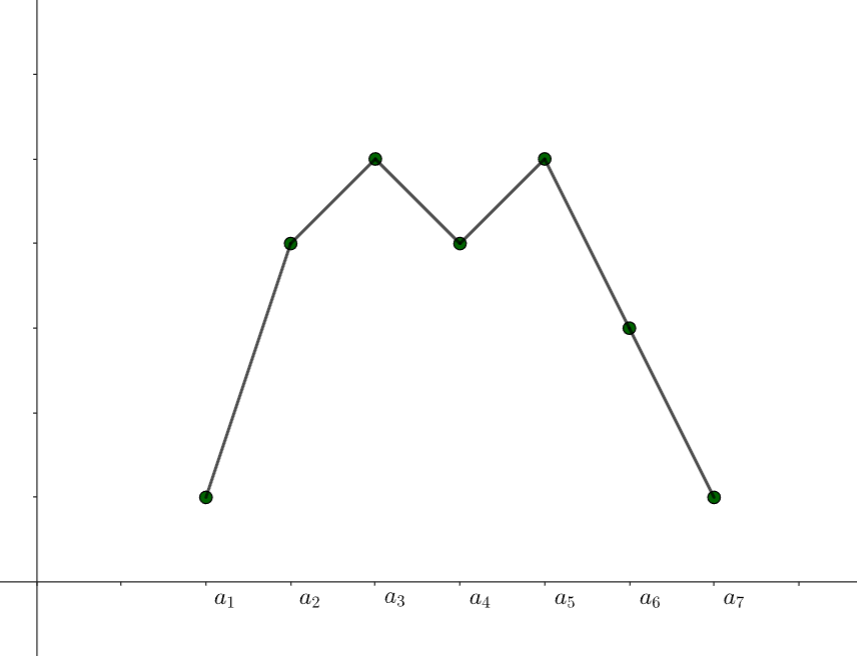
\includegraphics[width=0.7\textwidth]{mathstat/images/mathstat_2025_02_11_2}
    \end{center}

    \item Выборочная функция распределения

    На основе таблицы строится график функции распределения

    \begin{center}
        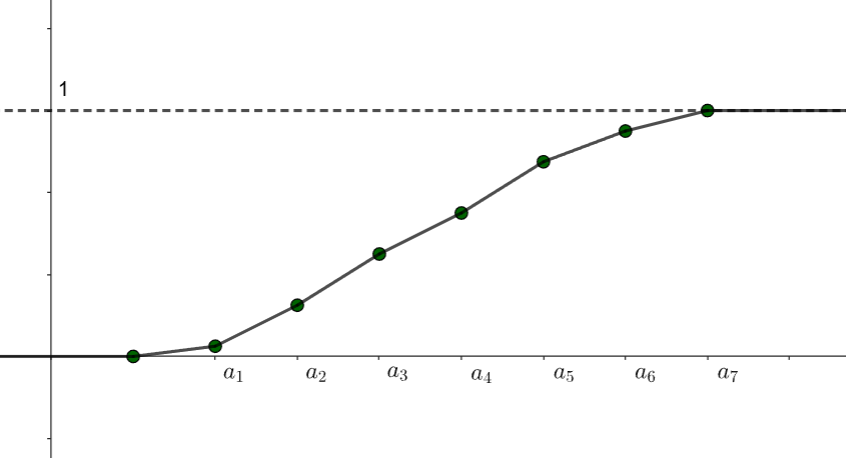
\includegraphics[width=0.7\textwidth]{mathstat/images/mathstat_2025_02_11_3}
    \end{center}

    Она может быть ступенчатой, ломаной или соединена по усмотрению

\end{itemize}





% end mathstat_2025_02_11.tex

% begin mathstat_2025_02_18.tex





\section{Лекция 2.}

\subsection{Точечная оценка}

Пусть имеется выборка $\vec{X} = (X_1, X_2, \dots, X_n)$ объемом $n$

Пусть требуется найти приближенную оценку $\theta^*$ неизвестного параметра $\theta$

Находим ее при помощи некоторой функции обработки данных $\theta^* = \theta^*(X_1, \dots, X_n)$

\Def Такая функция называется статистикой

\Defs А оценка $\theta^*$ называется точечной оценкой

\subsubsection{Свойство точечных оценок}

\begin{enumerate}
    \item Состоятельность

    \Defs Статистика $\theta^* = \theta^*(X_1, \dots, X_n)$ неизвестного параметра называется
    состоятельной, если $\theta^* \overset{p}{\longrightarrow} \theta$ при $n \to \infty$

    \mediumvspace

    \item Несмещенность

    \Defs Оценка $\theta^*$ параметра $\theta$ называется несмещенной, если 
    математическое ожидание $E \theta^* = \theta$
    
    \Notas Оценка $\theta^*$ называется асимптотически несмещенной, если 
    $E \theta^* \overset{p}{\longrightarrow} \theta$ при $n \to \infty$

    \mediumvspace

    \item Эффективность 

    \Defs Оценка $\theta^*_1$ не хуже $\theta^*_2$, если $E (\theta^*_1 - \theta)^2 \leq E (\theta^*_2 - \theta)^2$.
    Или, если $\theta^*_1$ и $\theta^*_2$ несмещенные, то $D \theta^*_1 \leq D \theta^*_2$

    \Defs Оценка $\theta^*$ называется эффективной, если она не хуже всех остальных оценок

    \Notas Не существует эффективной оценки в классе всех возможных оценок

    \begin{MyTheorem}
        \Ths В классе несмещенных оценок существует эффективная оценка
    \end{MyTheorem}

    \mediumvspace

    \item Асимптотическая нормальность

    \Defs Оценка $\theta^*$ параметра $\theta$ называется асимптотически нормальной, если 
    $\sqrt{n} (\theta^* - \theta) \rightrightarrows N(0, \sigma^2 (\theta))$ при $n \to \infty$
    
\end{enumerate}

\subsection{Точечные оценки моментов}

\Def Выборочным средним $\overline{x}$ называется величина $\overline{x} = \frac{1}{n} \sum_{i = 1}^n X_i$

\Defs Выборочной дисперсией $D^*$ называется величина $D^* = \frac{1}{n} \sum_{i = 1}^n (X_i - \overline{x})^2$

\Defs Исправленной дисперсией $S^2$ называется величина $S^2 = \frac{n}{n - 1} D^* = \frac{1}{n - 1} \sum_{i = 1}^n (X_i - \overline{x})^2$

\Defs Выборочным средним квадратическим отклонением называется величина $\sigma^* = \sqrt{D^*}$

\Defs Исправленным средним квадратическим отклонением называется величина $S = \sqrt{S^2}$

\Defs Выборочным $k$-ым моментом называется величина $\overline{x^k} = \frac{1}{n} \sum_{i = 1}^n X_i^k$

\Defs Модой $\mathrm{Mo}^*$ называется варианта $x_k$ с наибольшей частотой $n_k = \max_i (n_1, n_2, \dots, n_m)$

\Defs Выборочной медианой $\mathrm{Me}^*$ называется варианта $x_i$ в середине вариационного ряда $\begin{cases}\mathrm{Me}^* = 
X_{(k)}, & \text{если } n = 2k - 1 \\ \frac{X_{(k)} + X_{(k + 1)}}{2}, & \text{если } n = 2k\end{cases}$

\begin{MyTheorem}
    \Ths $\overline{x}$ - состоятельная несмещенная оценка теоретического матожидания $ЕX = a$

    1) $E \overline{x} = a$

    2) $\overline{x} \overset{p}{\longrightarrow} a$ при $n \to \infty$
\end{MyTheorem}

\begin{MyProof}
    1) $E \overline{x} = E\left(\frac{X_1 + \dots + X_n}{n}\right) = \frac{1}{n} \sum_{i = 1}^n E X_i = 
    \frac{1}{n} n E X_1 = E X_1 = a$

    2) $\overline{x} = \frac{\overline{x}_1 + \dots + \overline{x}_n}{n} \overset{p}{\longrightarrow} a$ 
    согласно Закону Больших Чисел
\end{MyProof}

\Nota Если второй момент конечен, то $\overline{x}$ - асимптотически нормальная оценка. По ЦПТ $\frac{S_n - n E X_1}{\sqrt{n} \sqrt{D X_1}} = \sqrt{n} \frac{\overline{x} - E X_1}{\sqrt{D X_1}} \rightrightarrows N(0, 1)$
или $\sqrt{n} (\overline{x} - E X_1) \rightrightarrows N(0; D X_1)$

\begin{MyTheorem}
    \Ths Выборочный $k$-ый момент является состоятельной несмещенной оценкой теоретического $k$-ого момента

    1) $\overline{E X^k} = E X^k$

    2) $\overline{X^k} \overset{p}{\longrightarrow} X^k$
\end{MyTheorem}

Это следует из предыдущей теоремы, если взять $X^k$ вместо $X$

\begin{MyTheorem}
    \Ths Выборочной дисперсией $D^*$ и $S^2$ являются состоятельными оценками теоретической дисперсией, при этом $D^*$ - смещенная оценка, а
    $S^2$ - несмещенная оценка
\end{MyTheorem}

\begin{MyProof}
    Заметим, что $D^* = \overline{X^2} - \overline{X}^2$

    $E D^* = E(\overline{X^2} - \overline{X}^2) = E\overline{X^2} - E (\overline{X}^2) = 
    E X^2 - E (\overline{X}^2)$

    Так как $D \overline{X} = E(\overline{X^2}) - (E \overline{X})^2$, то $E X^2 - E (\overline{X}^2) = 
    E X^2 - ((E\overline{X})^2 + D\overline{X}) = (E X^2 - EX) - D\overline{X} = D X - D \overline{X} = D X - D \left(\frac{X_1 + \dots + X_n}{n}\right) = 
    DX - \frac{1}{n^2} \sum_{i = 1}^n D X_i = DX - \frac{1}{n^2} n D X_1 = DX - \frac{1}{n} DX = \frac{n - 1}{n} DX$, то есть $D^*$ - смещенная вниз оценка

    $E S^2 = E(\frac{n}{n - 1} D^*) = \frac{n}{n - 1} \frac{n - 1}{n} DX = DX \Longrightarrow S^2$ - несмещенная вниз оценка 

    2. $D^* = \overline{X^2} - \overline{X}^2 \overset{p}{\longrightarrow} E X^2 - (E X)^2 = DX$ - состоятельная оценка

    $S^2 = \frac{n}{n - 1} D^* \overset{p}{\longrightarrow} DX$
\end{MyProof}

\Nota Отсюда видим, что выборочная дисперсия - асимптотически несмещенная оценка. Поэтому при большом (обычно не меньше 100) объеме выборке можно
считать обычную выборочную дисперсию

\subsection{Метод моментов (Пирсона)}

Постановка задачи: пусть имеется выборка объема $n$ неизвестного распределения, но известного типа,
которое задается $k$ параметрами: $\theta = (\theta_1, \theta_2, \dots, \theta_k)$. Требуется дать оценки данным
неизвестным параметрам

Идея метода состоит в том, что сначала находим оценки $k$ моментов, а затем с помощью теоретических формул
из теории вероятности даем оценки этих параметров

Пусть $\vec{X}$ - выборка из абсолютно непрерывного распределения $F_\theta$ с плотностью известного типа, 
которая задается $k$ параметрами $f_\theta (x, \theta_1, \dots, \theta_k)$

Тогда теоретические моменты находим по формуле $m_i = \int_{-\infty}^{\infty} x^i f_\theta (x, \theta_1, \dots, \theta_k) dx = h_i(\theta_1, \dots, \theta_n)$

Получаем систему из $k$ уравнений с $k$ неизвестными. В эти уравнения подставляем найденные оценки
моментов и, решая получившуюся систему уравнений, находим нужные оценки параметров

$\begin{cases}
    \overline{x} = h_1(\theta_1^*, \dots, \theta_n^*) \\ 
    \overline{x^2} = h_2(\theta_1^*, \dots, \theta_n^*) \\ 
    \dots \\
    \overline{x^k} = h_k(\theta_1^*, \dots, \theta_n^*) \\ 
\end{cases}$

\Nota Оценки по методу моментов как правило состоятельные, но часто смещенные

\Ex Пусть $X \in U(a, b)$. Обработав статданные, нашли оценки первого и второго моментов:

$\overline{x} = 2.25; \overline{x^2} = 6.75$

Найти оценки параметров $a^*, b^*$

Плотность равномерного распределения $f_{(a, b)} (x) = \begin{cases}0, & x < a \\ \frac{1}{b - a} & a \leq x \leq b, \\ 0, x > b\end{cases}$

$EX = \int_a^b x \frac{1}{b - a} dx = \frac{a + b}{2}$

$EX = \int_a^b x^2 \frac{1}{b - a} dx = \frac{a^2 + ab + b^2}{3}$

\mediumvspace

Получаем:

$\begin{cases}
    \overline{x} = \frac{a^* + b^*}{2} \\ 
    \overline{x^2} = \frac{a^*^2 + a^* b^* + b^*^2}{3} \\ 
\end{cases} \Longleftrightarrow \begin{cases}
    \frac{a^* + b^*}{2} = 4.5 \\ 
    a^*^2 + a^* b^* + b^*^2 = 20.25 \\ 
\end{cases} \Longleftrightarrow \begin{cases}
    \frac{a^* + b^*}{2} = 4.5 \\ 
    a^* b^* = 0 \\ 
\end{cases} \Longleftrightarrow \begin{cases}
    a^* = 0 \\ 
    b^* = 4.5 \\ 
\end{cases}$




% end mathstat_2025_02_18.tex

% begin mathstat_2025_02_25.tex





\section{Лекция 3.}

\subsection{Метод максимального правдоподобия}

Пусть имеется выборка $\vec{X} = (X_1, \dots, X_n)$ из распределения известного типа, определяемого неизвестными параметрами 
$\theta = (\theta_1, \dots, \theta_n)$

Идея метода состоит в следующем: подбираем параметры таким образом, чтобы вероятность получения
данной выборки при случайном эксперименте была наибольшей.

Если распределение дискретное, то $P_{\theta} (X_1 = x_1, X_2 = x_2, \dots, X_n = x_n) = P(X_1 = x_1) \dots P(X_n = x_n)$

\Def Функцией правдоподобия $L(\vec{X}, \theta)$ называется функция $L(\vec{X}, \theta) = P(X_1 = x_1) \dots P(X_n = x_n) = \prod_{i = 1}^n P(X_i = x_i)$ при дискретном распределении

и $L(\vec{X}, \theta) = f_\theta(x_1) \dots f_\theta(x_n) = \prod_{i = 1}^n f_\theta(x_i)$ в абсолютно непрерывном распределении

\Def Логарифмической функцией правдоподобия называется функция $\ln L(\vec{X}, \theta)$

\Nota Так как $y = \ln x$ возврастающая функция, точки максимума совпадают, а такую функцию правдоподобия становится легче дифференцировать

\Def Оценкой максимального правдоподобия $\hat{\theta}$ называется значение $\theta$, при котором функция правдоподобия 
$L(\vec{X}, \theta)$ достигает наибольшего значения (при фиксированных значениях выборки)

\ExN{1} Пусть $\vec{X} = (X_1, \dots, X_n)$ - выборка из распределения Пуассона $\Pi_\lambda$ с неизвестным $\lambda > 0$

\Mem Для распределения Пуассона $P(X = x_i) = \frac{\lambda^{x_i}}{x_i!} e^{-\lambda}$

Получаем функцию максимального правдоподобия $L(\vec{X}, \lambda) = \prod_{i = 1}^n \frac{\lambda^{x_i}}{x_i!} e^{-\lambda} = 
\frac{\lambda^{\sum_{i = 1}^n x_i}}{\prod_{i = 1}^n x_i!} e^{-n\lambda} = \frac{\lambda^{n \overline{x}}}{\prod_{i = 1}^n x_i!} e^{-n\lambda}$

$\ln L(\vec{X}, \lambda) = n \overline{x} \ln \lambda - \ln \prod_{i = 1}^n x_i! - n\lambda$

$\frac{\partial \ln L}{\partial \lambda} = \frac{n \overline{x}}{\lambda} - n = 0 \Longrightarrow \hat{\lambda} = \overline{x}$ - оценка максимального правдоподобия

Убедимся, что этот экстремум - максимум: $\frac{\partial^2 \ln L}{\partial \lambda^2} = -\frac{n \overline{x}}{\lambda} < 0 \Longrightarrow \hat{\lambda} = \overline{x}$ - точка максимума

\ExN{2} Пусть $(X_1, \dots, X_n)$ из $N(a, \sigma^2)$

$f_{a, \sigma^2} (x) = \frac{1}{\sigma \sqrt{2\pi}} e^{-\frac{(x - a)^2}{2\sigma^2}}$

$L(\vec{X}, a, \sigma^2) = \prod_{i = 1}^n \frac{1}{\sigma \sqrt{2\pi}} e^{-\frac{(x_i - a)^2}{2\sigma^2}} = 
\frac{1}{\sigma^n (2\pi)^{\frac{n}{2}}} e^{-\frac{\sum_{i = 1}^n (x_i - a)^2}{2\sigma^2}}$

$\ln L(\vec{X}, a, \sigma^2) = -n\ln \sigma - \frac{n}{2} \ln 2\pi - \frac{1}{2\sigma^2}\sum_{i = 1}^n (x_i - a)^2$

$\frac{\partial \ln L}{\partial a} = -\frac{1}{2\sigma^2} \sum_{i = 1}^n -2(x_i - a) = \frac{1}{\sigma^2} \sum_{i = 1}^n (x_i - a) = \frac{n\overline{x} - na}{\sigma^2}$

$\frac{\partial \ln L}{\partial \sigma} = -\frac{n}{\sigma} - \sum_{i = 1}^n (x_i - a)^2 \frac{1}{2} \cdot (-2) \cdot \sigma^{-3} = \frac{1}{\sigma^3} \sum_{i = 1}^n (x_i - a)^2 - \frac{n}{\sigma}$

$\begin{cases}
    \frac{n\overline{x} - na}{\sigma^2} = 0 \\
    \frac{1}{\sigma^3} \sum_{i = 1}^n (x_i - a)^2 - \frac{n}{\sigma} = 0
\end{cases} \Longrightarrow \begin{cases}
    \hat{a} = \overline{x} \\
    \widehat{\sigma^2} = \frac{1}{n} \sum_{i = 1}^n (x_i - a)^2 = D^*
\end{cases} $

\ExN{3} Пусть $(X_1, \dots, X_n)$ из $U(0, \theta)$. Найти оценку $\theta$ этого распределения.

Воспользуемся методом моментов:

$EX = \frac{a + b}{2} = \frac{\theta}{2} \Longrightarrow \overline{x} = \frac{\theta^*}{2} \Longrightarrow \theta^* = 2\overline{x}$

Воспользуемся методом максимального правдоподобия:

$f_\theta = \begin{cases}0, & x < 0 \\ \frac{1}{\theta}, & 0 \leq x \leq \theta \\ 0, & x > \theta \end{cases}$

$X_{(n)} = \max_i (X_1, \dots, X_n)$

$L(\vec{X}, \theta) = \prod_{i = 1}^n f_\theta (x_i) = 
\begin{cases}
    0, & \text{если } \theta < X_{(n)} \\ 
    \frac{1}{\theta^n}, & \text{если } \theta \geq X_{(n)}
\end{cases}$

$L(\vec{X}, \theta)$ достигает наибольшего значения при наименьшем значении $\theta^n$, то есть при $\hat{\theta} = X_{(n)}$

Сравним оценки:

$\theta^* = 2 \overline{x}$ - несмещенная оценка, так как $E\theta^* = 2E\overline{x} = 2E X = \theta$

$E(\theta^* - \theta)^2 = D\theta^* = D2\overline{x} = 4D\overline{x} = 4\frac{D\overline{x}}{n} = \frac{4}{n}\frac{\theta^2}{12} = \frac{\theta^2}{3n}$

Изучим распределение $X_{(n)}$: $F_{X_{(n)}}(x) = P(X_{(n)} < x) = P(X_1 < x, X_2 < x, \dots, X_n < x) = 
P(X_1 < x) \dots P(X_n < x) = F_{X_1}(x) \dots F_{X_n}(x) = F^n_{(x_1)}(x)$

$F_{X_1} (x) = \begin{cases}
    0, & x < 0 \\
    \frac{x}{\theta}, & 0 \leq x \leq \theta \\
    1, & x > \theta
\end{cases} \Longrightarrow F_{X_(n)}(x) = \begin{cases}
    0, & x < 0 \\
    \frac{x^n}{\theta^n}, & 0 \leq x \leq \theta \\
    1, & x > \theta
\end{cases} \Longrightarrow f_{X_(n)}(x) = \begin{cases}
    0, & x < 0 \\
    n\frac{x^{n - 1}}{\theta^n}, & 0 \leq x \leq \theta \\
    1, & x > \theta
\end{cases}$

$EX_{(n)} = \int_0^\theta x \cdot \frac{nx^{n - 1}}{\theta^n} dx = \frac{n}{\theta^n} \int_0^\theta x^n dx = \frac{n x^{x + 1}}{\theta^n (n + 1)} \Big|_0^\theta = 
\frac{n\theta}{n + 1}$ - смещенная вниз оценка

$\tilde{\theta} = \frac{n + 1}{n} X_{(n)}$ - несмещенная оценка (будем считать, что эффективность не изменилась)

$E\tilde{\theta}^2 = E(\frac{n + 1}{n} X_{(n)})^2 = \frac{(x + 1)^2}{n^2} E X_{(n)} = \frac{(n + 1)^2}{n^2} \int_0^\theta x^2 \frac{n x^{n - 1}}{\theta^n} dx = 
\frac{(n + 1)^2 \theta^2}{n (n + 2)}$

$D\tilde{\theta} = E\tilde{\theta}^2 - (E\tilde{\theta})^2 = \frac{\theta^2}{n(n + 2)}$

$D\tilde{\theta} = \frac{\theta^2}{n(n + 2)} < \frac{\theta^2}{3n} = D\theta^*$

Таким образом, оценка по методу правдоподобия сходится быстрее, чем оценка по методу моментов, поэтому она лучше

Отсюда следует, что при равномерном распределении выборочное среднее не является эффективной оценкой
для математического ожидания; вместо нее половина максимального элемента выборки будет лучше

\Nota Эффективной здесь будет несмещенная оценка $\frac{n + 1}{2n} X_{(n)}$

В общем случае для $U(a, b)$ будет такая эффективная оценка матожидания - $\frac{X_{(1)} + X_{(n)}}{2}$, длины интервала - $\frac{n + 1}{n - 1} (X_{(n)} - X_{(1)})$

\Nota При методе максимального правдоподобия обычно получаем состоятельные и эффективные оценки, но часто смещенные

\subsection{Неравенство Рао-Крамера}

Пусть $X \in F_\theta$ - семейство распределений с параметром $\theta \in \Real$

\Def Носителем семейства распределений $F_\theta$ называется множество $C \subset \Real$
такое, что $P(X \in C) = 1 \ \forall X \in F_\theta$

$f_\theta(x) = \begin{cases}
    \text{плотность } f_\theta(x) \text{ при непрерывном распределении} \\
    P_\theta(X = x) \text{ при дискретном распределении}
\end{cases}$

\Def Информацией Фишера $I(\theta)$ семейства распределений $F_\theta$ называется величина 
$I(\theta) = E\left(\frac{\partial}{\partial \theta} \ln f_\theta(X)\right)^2$ при условии, что
она существует

\Def Семейство распределений $F_\theta$ называется регулярным, если:

\begin{itemize}
    \item существует носитель $C$ семейства $F_\theta$ такой, что $\forall x \in C \ $ функция $\ln f_\theta(x)$ непрерывно дифференцируема по $\theta$
    \item информация Фишера $I(\theta)$ существует и непрерывна по $\theta$
\end{itemize}

\begin{MyTheorem}
    \Ths Пусть $(X_1, \dots, X_n)$ - выборка объема $n$ из регулярного семейства $F_\theta$,

    $\theta^* = \theta^*(X_1, \dots, X_n)$ - несмещенная оценка параметра $\theta$, дисперсия которой
    $D\theta^*$ ограничена в любой замкнутой ограниченной области параметра $\theta$

    Тогда \fbox{$D\theta^* \geq \frac{1}{n I(\theta)}$}
\end{MyTheorem}

\underline{Следствие}: если при данных услових получили $D\theta^* = \frac{1}{n I(\theta)}$, то оценка $\theta^*$ является эффективной 
(то есть дальше улучшать уже некуда)

\Ex Пусть $(X_1, \dots, X_n)$ из $N(a, \sigma^2)$ (то есть $F_a = N(a, \sigma^2)$, $\sigma^2$ зафиксируем)

Проверим эффективность $a^* = \overline{x}$

Плотность $f_a(x) = \frac{1}{\sigma \sqrt{2\pi}} e^{-\frac{(x - a)^2}{2\sigma^2}}$, носитель - вся прямая $\Real$

$\ln f_a(x) = -\ln \sigma - \frac{1}{2} \ln 2\pi - \frac{(x - a)^2}{2\sigma^2}, \quad\quad a \in (-\infty, \infty)$

$\frac{\partial}{\partial a} \ln f_a(x) = \frac{1}{2\sigma^2} \cdot 2(x - a) = \frac{x - a}{\sigma^2}$ - непрерывна для всех $a \in \Real$

$I(a) = E\left(\frac{\partial}{\partial a} \ln f_a(X)\right)^2 = E\left(\frac{X - a}{\sigma^2}\right)^2 = \frac{1}{\sigma^4} E(X - a)^2 = \frac{E(X - EX)^2}{\sigma^4} = 
\frac{DX}{\sigma^4} = \frac{1}{\sigma^2}$ - непрерывна по $a$

Из этого следует, что $N(a, \sigma^2)$ - регулярное семейство относительно параметра $a$

$Da^* = D\overline{x} = \frac{DX}{n} = \frac{\sigma^2}{n}$ - ограничена по параметру $a$

По неравенству Рао-Крамера $Da^* = \frac{\sigma^2}{n} =\joinrel= \frac{1}{nI(a)} = \frac{1}{n} \sigma^2$; из 
этого следует, что $a^*$ - эффективная оценка параметра $a$

\Nota Аналогично можно показать, что $S^2$ - несмещенная эффективная оценка для параметра $\sigma^2$



% end mathstat_2025_02_25.tex

% begin mathstat_2025_03_04.tex





\section{Лекция 4.}

\subsection{Основные распределения математической статистики}

\Def Случайная величина имеет нормальное распределение $\xi \in N(a, \sigma^2)$ с параметрами $a$ и $\sigma^2$, если
ее плотность имеет вид $f_\xi(x) = \frac{1}{\sigma\sqrt{2\pi}} e^{-\frac{(x - a)^2}{2\sigma^2}}$

На практике нормальное распределение встречается чаще всего в силу ЦПТ

\Def Распределение $N(0, 1)$ с параметрами $a = 0, \sigma^2 = 1$ называется стандартным нормальным распределением. 
Его плотность равна $\varphi(x) = \frac{1}{\sqrt{2\pi}} e^{-\frac{x^2}{2}}$. 
В дальнейшем такую случайную величину будем называть стандартной нормалью

\underline{Свойства}

\begin{enumerate}
    \item $a = E\xi \qquad \sigma^2 = D\xi$

    \item Линейность: $\xi \in N(a, \sigma^2)$, то $\eta = b \xi + \gamma \in N(ab + \gamma, b^2 \sigma^2)$

    \item Стандартизация: Если $\xi \in N(a, \sigma^2)$, то $\eta = \frac{\xi - a}{\sigma} \in N(0, 1)$

    \item Устойчивость относительно суммирования: если $\xi_1 \in N(a_1, \sigma^2_1)$, $\xi_2 \in N(a_2, \sigma^2_2)$, независимы
    то $\xi_1 + \xi_2 \in N(a_1 + a_2, \sigma^2_1 + \sigma^2_2)$
\end{enumerate}

\subsubsection{Распределение \enquote{хи-квадрат}}

\Def Распределение \enquote{хи-квадрат} $H_n$ со степенями свободы $n$ называется распределение
суммы квадратов независимых стандартных нормальных величин: $\xi^2_n = X_1^2 + X_2^2 + \dots + X_n^2$, 
где $X \in N(0, 1)$ и независимы

\underline{Свойства}

\begin{enumerate}
    \item $E\xi^2_n = n$

    \begin{MyProof}
        Так как $\forall i \ X_i \in N(0, 1)$, то $E X_i^2 = D X_i^2 + (EX_i)^2 = 1 \Longrightarrow E(X_i^2 + \dots X_n^2) = \sum_{i = 1}^n X_i^2 = n$
    \end{MyProof}

    \item Устойчивость относительно суммирования: если $X \in H_n$, $Y \in H_m$, независимы, то $X + Y \in H_{n + m}$ (по определению) 


    \item $\frac{\xi_k^2}{k} \overset{p}{\underset{k \to \infty}{\longrightarrow}} 1$ (по Закону Больших Чисел)
\end{enumerate}

\subsubsection{Распределение Стьюдента}

\Def Пусть $X_0, X_1, \dots, X_k$ - независимые стандартные нормальные величины. 
Распределением Стьюдента $T_k$ с $k$ степенями свободы называется распределение случайной величины 
$t_k = \frac{X_0}{\sqrt{\frac{1}{k}} (X_0^2 + \dots + X_k^2)} = \frac{X_0}{\sqrt{\frac{\xi_k^2}{k}}}$

\underline{Свойства}

\begin{enumerate}
    \item $Et_k = 0$ - в силу симметрии

    \item $t_k \rightrightarrows N(0, 1)$ (на практике при $k \geq 100$ распределение Стьюдента можно считать стандартным нормальным)
\end{enumerate}

\subsubsection{Распределение Фишера-Снедекера}

\Def Распределением Фишера-Снедекера $F_{n,m}$ (другое название - F-распределение) со степенями свободы $n$ и $m$ называется распределение случайной величины 
$f_{n,m} = \frac{\frac{\xi^2_n}{n}}{\frac{\xi^2_m}{m}}$, где $\xi_n^2$ и $\xi_m^2$ - независимые случайные величины с распределением \enquote{хи-квадрат}

\underline{Свойства}

\begin{enumerate}
    \item $E f_{n,m} = \frac{n}{n - 2}$

    \item $f_{n,m} \overset{p}{\underset{n, m \to \infty}{\longrightarrow}} 1$
\end{enumerate}


\subsection{Математическое ожидание и дисперсия случайного вектора}

Пусть $\vec X = \begin{pmatrix}X_1 \\ \vdots \\ X_n\end{pmatrix}$ - случайный вектор, 
где случайная величина $X_i$ - компонента (координата) случайного вектора

\Def Математическим ожидание случайного вектора называется вектор с координатами из математических ожиданий компонент: 
$E \vec X = \begin{pmatrix}E X_1 \\ \vdots \\ E X_n\end{pmatrix}$

\Def Дисперсией случайного вектора (или матрицей ковариаций) случайного вектора $\vec X$ называется
матрица $D \vec X = E (\vec X - E \vec X) (\vec X - E \vec X)^T$, состоящая из элементов $d_{ij} = \cov (X_i, X_j)$

\Notas На главной диагонали стоят дисперсии компонент: $d_{ii} = D X_i$

\Notas $D \vec X$ - симметричная положительно определенная матрица

\underline{Свойства}

\begin{enumerate}
    \item $E (A \vec X) = A E \vec X$

    \item $E (\vec X + \vec B) = E \vec X + \vec B$, где $\vec B$ - вектор чисел

    \item $D (A \vec X) = A \cdot D \vec X \cdot A^T$

    \item $D (\vec X + \vec B) = D \vec X$
\end{enumerate}

\subsection{Многомерное нормальное распределение}

\Def Пусть случайный вектор $\vec \xi = \begin{pmatrix}\xi_1 \\ \vdots \\ \xi_n\end{pmatrix}$ имеет вектор средних 
$\vec a = E \vec \xi$, $K$ - симметричная положительно определенная матрица. Вектор $\vec \xi$ 
имеет нормальное распределение в $\Real^n$ с параметрами $\vec a$ и $K$, если его плотность 
$f_{\vec \xi} (\vec X) = \frac{1}{\left(\sqrt{2\pi}\right)^n \sqrt{\det K}} e^{-\frac{1}{2} (\vec X - \vec a)^T K^{-1} (\vec X - \vec a)}$


\underline{Свойства}

\begin{enumerate}
    \item Матрица $K = D \vec \xi = \left(\cov (\xi_i, \xi_j)\right)$ - матрица ковариаций

    \item При $\vec a = \vec 0$ и $K = E$ имеем вектор из независимых стандартных нормальных величин

    \begin{MyProof}
        При $\vec a = \vec 0$ и $K = E$: $f_{\vec \xi} (X_1, \dots, X_n) = \frac{1}{\left(\sqrt{2\pi}\right)^n} 
        e^{-\frac{1}{2} \begin{pmatrix}X_1 & \dots & X_n\end{pmatrix} E \begin{pmatrix}X_1 & \dots & X_n\end{pmatrix}^T} = 
        \frac{1}{\left(\sqrt{2\pi}\right)^n} e^{-\frac{1}{2} (X_1^2 + \dots + X_n^2)} = 
        \frac{1}{\sqrt{2\pi}} e^{-\frac{1}{2} X_1^2} + \dots + \frac{1}{\sqrt{2\pi}} e^{-\frac{1}{2} X_n^2}$

        Так как плотность распалась на произведение плотностей стандартного нормального распределение, то все компоненты имеют стандартное нормальное распределение
    \end{MyProof}
\end{enumerate}

Далее вектором из независимых стандартных нормальных величин для краткости будем называть стандартным нормальным вектором

\begin{enumerate}
    \setcounter{enumi}{2}

    \item $\letsymbol \vec X$ - стандартный нормальный вектор, $B$ - невырожденная матрица, 
    тогда вектор $\vec Y = B \vec X + \vec a$ имеет многомерное нормальное распределение с параметрами $\vec a$ и $K = B B^T$

    \item $\letsymbol \vec Y \in N(\vec a, K)$. Тогда вектор $\vec X = B^{-1} (\vec Y - \vec a)$ - стандартный нормальный вектор, где $\sqrt{K}$

    \underline{Следствие}. Эквивалентное определение: Многомерное нормальное распределение - это то, которое получается из
    стандартного нормального вектора при помощи невырожденного преобразования и сдвиг

    \item $\letsymbol \vec X$ - стандартный нормальный вектор, $C$ - ортогональная матрица. Тогда $\vec Y = C \vec X$ - стандартный нормальный вектор

    \begin{MyProof}
        Так как $C$ - ортогональная, то $C^T = C^{-1}$. Тогда по третьему свойству $K = C C^T = E$, а по второму свойству $\vec Y$ - стандартный нормальный вектор
    \end{MyProof}

    \item $\letsymbol$ случайный вектор $\xi \in N(\vec a, K)$.
    Тогда его координаты независимы тогда и только тогда, когда они не коррелированы (то есть матрица ковариаций $K$ диагональная)

    % какого распределения величины
    \underline{Следствие}. Если плотность совместного распределения случайных величин $\xi$ и $\eta$ ненулевая, то они независимы тогда и только тогда, 
    когда их коэффициент корреляции равен нулю
\end{enumerate}

\subsection{Многомерная центральная предельная теорема}

\begin{MyTheorem} 
    \Ths Среднее арифметическое независимых одинаково распределенных случайных векторов слабо сходится к многомерному нормальному распределению
\end{MyTheorem}

\subsection{Лемма Фишера}

\begin{MyTheorem}
    Пусть вектор $\vec X$ - стандартный нормальный вектор, $C$ - ортогональная матрица, $\vec Y = C \vec X$.
    Тогда $\forall 1 \leq k \leq n - 1 \ $ случайная величина $T(\vec X) = \sum_{i = 1}^n X_i^2 - Y_1^2 - Y_2^2 - \dots Y_k^2$ 
    не зависит от $Y_1, Y_2, \dots, Y_k$ и имеет распределение \enquote{хи-квадрат} со степенями свободы $n - k$
\end{MyTheorem}

\begin{MyProof}
    Так как $C$ - ортогональное преобразование, то $\|\vec X\| = \|\vec Y\|$, то есть $\sum_{i = 1}^n X^2_i = \sum_{i = 1}^n Y^2_i \Longrightarrow
    T(\vec X) = \sum_{i = 1}^n X_i^2 - Y_1^2 - Y_2^2 - \dots Y_k^2 = Y^2_{k + 1} + \dots + Y^2_{n}$

    Согласно свойству 5 $Y_i \in N(0, 1)$ и независимы, то по определению \enquote{хи-квадрат} $T(\vec X) \in H_{n - k}$ и не зависит от $Y_1, \dots, Y_k$
\end{MyProof}

\subsection{Основная теорема}

\begin{MyTheorem}
    \Ths Пусть $(X_1, \dots, X_n)$ - выборка из нормального распределения $N(a, \sigma^2)$, $\overline{x}$ - выборочное среднее, $S^2$ - исправленная дисперсия.

    Тогда имеет место следующее распределение 

    \begin{enumerate}
        \item $\sqrt{n} \frac{\overline{x} - a}{\sigma} \in N(0, 1)$
        
        \item $\sum_{i = 1}^n \frac{(X_i - a)^2}{\sigma^2} \in H_n$
        
        \item $\sum_{i = 1}^n \frac{(X_i - \overline{x})^2}{\sigma^2} = \frac{n D^*}{\sigma^2} = \frac{(n - 1) S^2}{\sigma^2} \in H_{n - 1}$

        \item $\sqrt{n} \frac{\overline{x} - a}{S} \in T_{n - 1}$
        
        \item $\overline{x}$ и $S^2$ независимы
    \end{enumerate}
\end{MyTheorem}

\begin{MyProof}
    \begin{enumerate}
        \item Так как $X_i \in N(a, \sigma^2)$, то $\sum_{i = 1}^n X_i \in N(na, n\sigma^2) \Longrightarrow \overline{x} \in N\left(a, \frac{\sigma^2}{n}\right) \Longrightarrow
        \overline{x} - a \in N\left(0, \frac{\sigma^2}{n}\right) \Longrightarrow \frac{\sqrt{n}}{\sigma} (\overline{x} - a) \in N(0, 1)$

        \item Так как $X_i \in N(a, \sigma^2)$, то $\frac{x_i - a}{\sigma} \in N(0, 1)$ и $\sum_{i = 1}^n \left(\frac{(x_i - a)^2}{\sigma^2}\right)^2 \in H_n$ по определению
        
        \item $\sum_{i = 1}^n \left(\frac{(x_i - \overline{x})^2}{\sigma^2}\right)^2 = \sum_{i = 1}^n \left(\frac{x_i - a}{\sigma} - \frac{\overline{x} - a}{\sigma}\right)^2 = 
        \sum_{i = 1}^n (z_i - \overline{z})$, где $z_i = \frac{x_i - a}{\sigma} \in N(0, 1)$, $\overline{z} = \frac{1}{n} \sum_{i = 1}^n z_i = \frac{\sum_{i = 1}^n x_i - na}{\sigma} = \frac{\overline{x} - a}{\sigma}$

        Поэтому можно считать, что изначально $X_i \in N(0, 1)$

        $T(\vec X) = \sum_{i = 1}^n \left(X_i - \overline{x}\right)^2 = n D^* = n (\overline{x^2} - \overline{x}^2) = \sum_{i = 1}^n X_i^2 - n\overline{x}^2 = \sum_{i = 1}^n X_i^2 - Y_1^2$, где $Y_1 = \sqrt{n} \overline{x} = \frac{X_1}{\sqrt{n}} + \dots + \frac{X_n}{\sqrt{n}}$

        Строчка $(\frac{1}{\sqrt{n}}, \dots, \frac{1}{\sqrt{n}})$ имеет длину 1, поэтому ее можно дополнить до ортогональной матрицы $C$, тогда $Y_1$ - первая компонента $\vec Y = C \vec X$, 
        и согласно лемме Фишера $T(\vec X) = \sum_{i = 1}^n (X_i - \overline{X})^2 \in H_{n - 1}$

        
        \setcounter{enumi}{4}
        \item Согласно лемме Фишера $T(\vec X) = (n - 1) S^2$ не зависит от $Y_1 = \sqrt{n} \overline{x} \Longrightarrow S^2 $ и $\overline{x}$ - независимы
          
        \setcounter{enumi}{3}
        \item $\sqrt{n} \frac{\overline{x} - a}{S} = \sqrt{n} \frac{\overline{x} - a}{\sigma} \cdot \frac{1}{\sqrt{\frac{S^2 (n - 1)}{\sigma^2}} \cdot \frac{1}{n - 1}} = \frac{\sqrt{n} \frac{\overline{x} - a}{\sigma}}{\frac{\xi^2_{n - 1}}{n - 1}}$

        Так как по пятому пункту числитель и знаменатель независимы, по определению получаем распределение Стьюдента
    \end{enumerate}
\end{MyProof}






% end mathstat_2025_03_04.tex



\end{document}

